%
% variation.tex
%
% (c) 2021 Prof Dr Andreas Müller, OST Ostschweizer Fachhochschule
%
\documentclass[tikz]{standalone}
\usepackage{times}
\usepackage{amsmath}
\usepackage{txfonts}
\usepackage[utf8]{inputenc}
\usepackage{graphics}
\usetikzlibrary{arrows,intersections,math}
\definecolor{flaechefarbe}{rgb}{1.0,0.4,0.8}
\definecolor{variationfarbe}{rgb}{0.4,0.8,0.8}
\usepackage{ifthen}
\begin{document}

\newboolean{showgrid}
\setboolean{showgrid}{false}
\def\breite{7}
\def\hoehe{4}

\def\achslabel{
	\node at (-3.00,-0.20) {$x\mathstrut$};
	\node at (3.08,-1.30) {$y\mathstrut$};
	\node at (-0.20,2.10) {$z\mathstrut$};
}

\begin{tikzpicture}[>=latex,thick]
\clip (-6.3,-2.2) rectangle (6.3,2.2);

% Povray Bild
\begin{scope}[xshift=-3.15cm]
\node at (0,0) {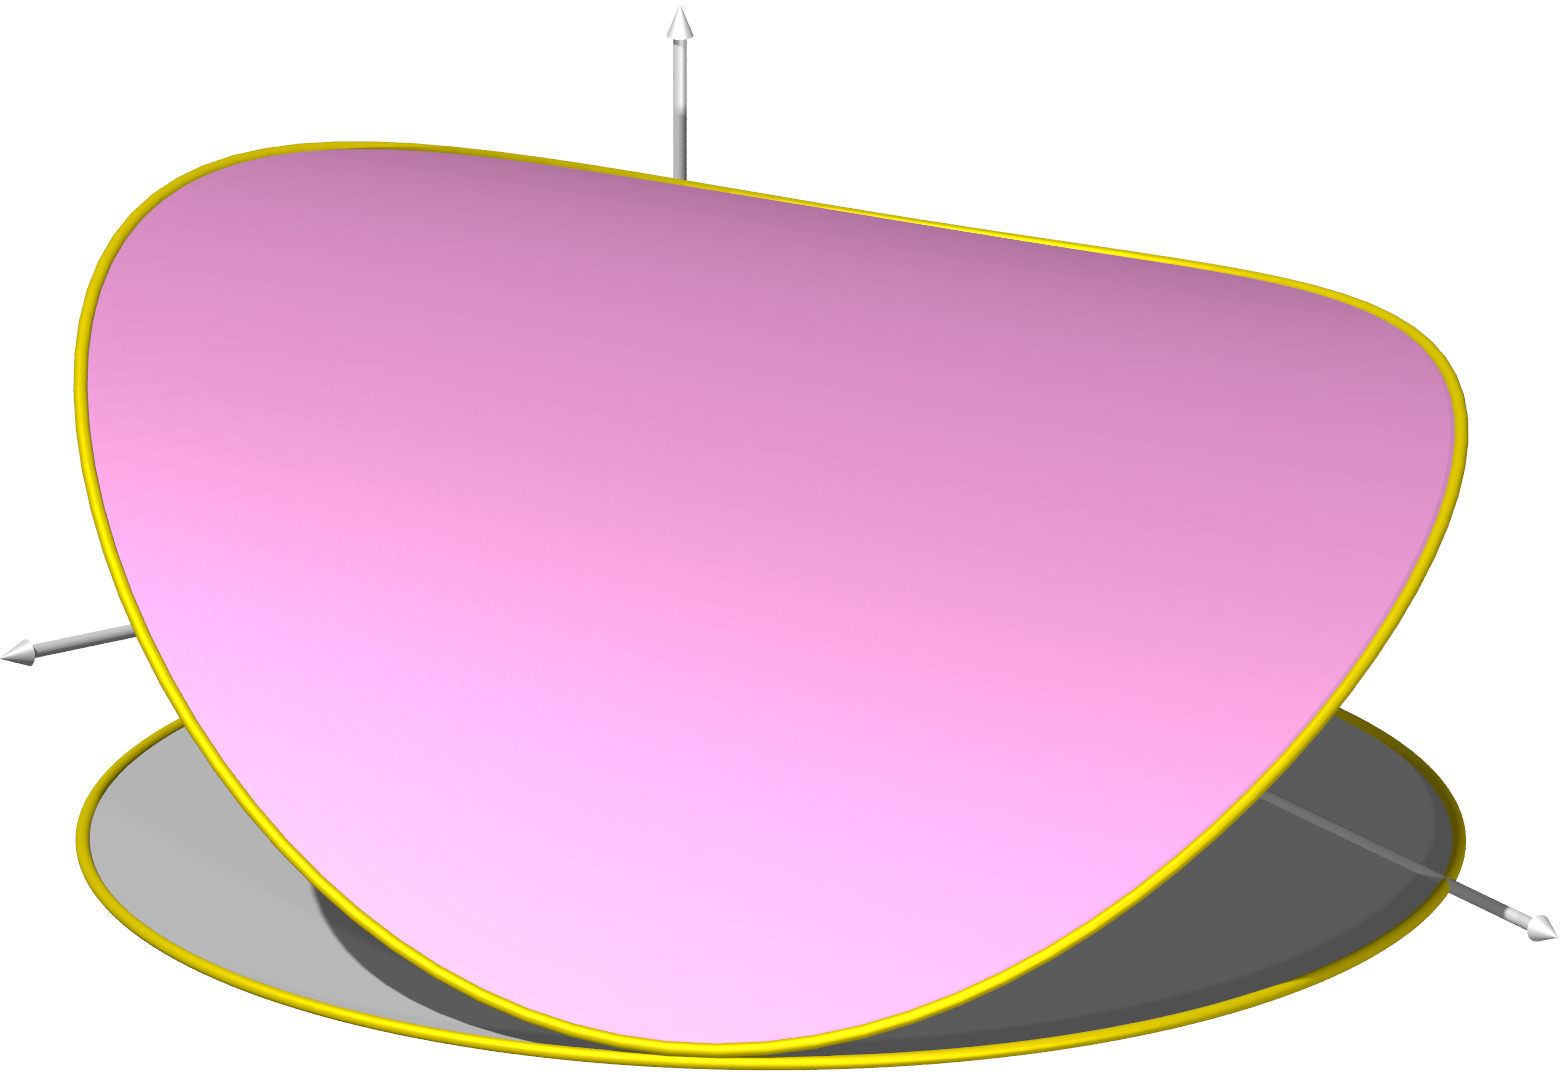
\includegraphics[width=6.3cm]{flaeche.jpg}};
\achslabel
\node at (0.00,0.00) {$z=\varphi(x,y)$};
\node at (-2.30,-1.30) {$\Omega$};
\end{scope}

\begin{scope}[xshift=3.15cm]
\node at (0,0) {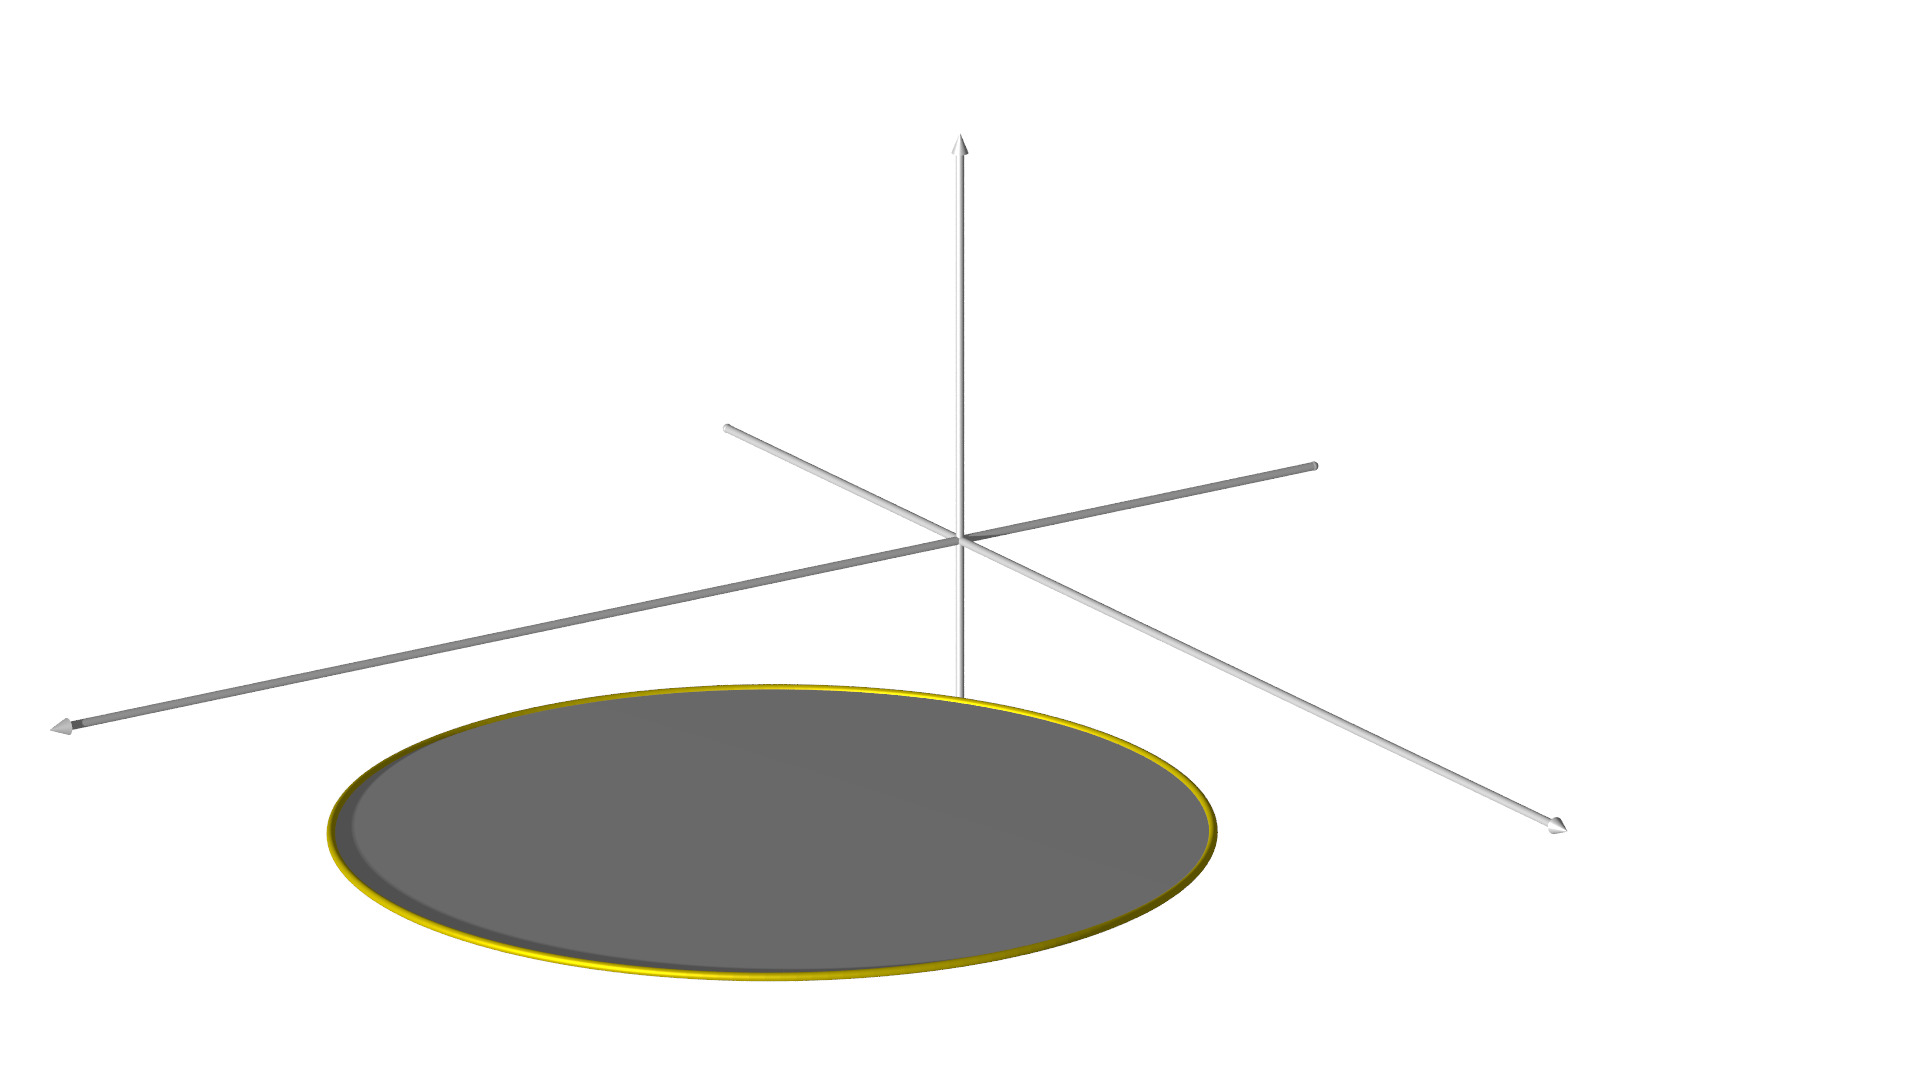
\includegraphics[width=6.3cm]{variation.jpg}};
\achslabel
\node at (1.30,1.60) {$z={\color{flaechefarbe}\varphi(x,y)}+\varepsilon{\color{variationfarbe}\eta(x,y)}$};
\node at (-0.10,-1.60) {$\Omega$};
\end{scope}

% Gitter
\ifthenelse{\boolean{showgrid}}{
\draw[step=0.1,line width=0.1pt] (-\breite,-\hoehe) grid (\breite, \hoehe);
\draw[step=0.5,line width=0.4pt] (-\breite,-\hoehe) grid (\breite, \hoehe);
\draw                            (-\breite,-\hoehe) grid (\breite, \hoehe);
\fill (0,0) circle[radius=0.05];
}{}

\end{tikzpicture}

\end{document}

